\subsection{Hyperledger Composer}
\label{sec:prototype_composer}
        Hyperledger Composer\cite{ComposerDocs} ist eine Abstraktion des Hyperledger Fabric Frameworks und dient vornehmlich für das Entwickeln von Blockchain-Netzwerken. 
        \medskip\\
        Composer bietet die Möglichkeit private Blockchainnetzwerke, genannt ,,Business Networks``, zu entwickeln und innerhalb eines Docker-Container zu betreiben.
        Weitere Werkzeuge des Frameworks können eine konfigurierbare \gls{rest}-\gls{api} und eine minimalistische Angular-Webapplikation generieren.
        \medskip\\
        Für die Entwicklung der Transaktionslogik von Business Networks wird die Sprache JavaScript verwendet. 
        Darüber hinaus werden domainspezifische Sprachen jeweils für die Modellierung der Teilnehmer im Netzwerk, sowie der Zugriffskontrolle und Anfragen and die Blockchain eingesetzt.
        \medskip\\
        Alle erfolgreichen Transaktionen von Assets werden im Ledger, gespeichert, wobei der aktuelle World State zusätzlich in einer Datenbank gespeichert wird. 
        Das Framework sorgt dafür, dass der Ledger und die Datenbank an alle Knoten verteilt wird und konsistent bleibt.\\
        Der ,,Historian`` schreibt zusätzlich alle weiteren Transaktionen wie das Hinzufügen oder Entfernen eines Teilnehmers in \colorbox{light-gray}{\lstinline{Historian Records}}, einem speziellen Typ von Asset, das ebenfalls in der Blockchain gespeichert wird.
        
        \subsubsection*{Aufbau}
        Ein Business Network besteht aus Assets, Participants, Transactions, \gls{acl}, optionalen Events und optionalen Queries.
        \begin{itemize}[noitemsep]
            \item \textbf{Assets}: Güter, die auf der Blockchain gespeichert werden
            \item \textbf{Participants}: Teilnehmer des Netzwerkes
            \item \textbf{Transactions}: Funktionen, die ausgeführt werden können, können Smart Contracts (sogenannte ,,Transaction Processor Functions``) auslösen, die  beliebige Aktionen ausführen können
            \item \textbf{Access Control Rules}: legen fest, welche Teilnehmer welche Aktionen im Netzwerk ausüben dürfen. 
                Zu vergebende Berechtigungen bestehen grundlegend aus einer Operation (CRUD\!\footnote{Create, Read, Update, Delete}), der betroffenen Ressource (Asset, Participant oder Transaction) und dem Akteur, der die Operation ausführt.
                Die Regeln werden sequentiell in geordneter Reihenfolge ausgewertet. 
        \end{itemize}
        Die einzelnen Bestandteile werden zu einem ,,Business Network Archive`` zusammengefasst und auf einer Hyperledger Fabric-Instanz ausgerollt (siehe \fref{fig:composer_arch}).
        
        \begin{figure}[H]
    		\centering
    		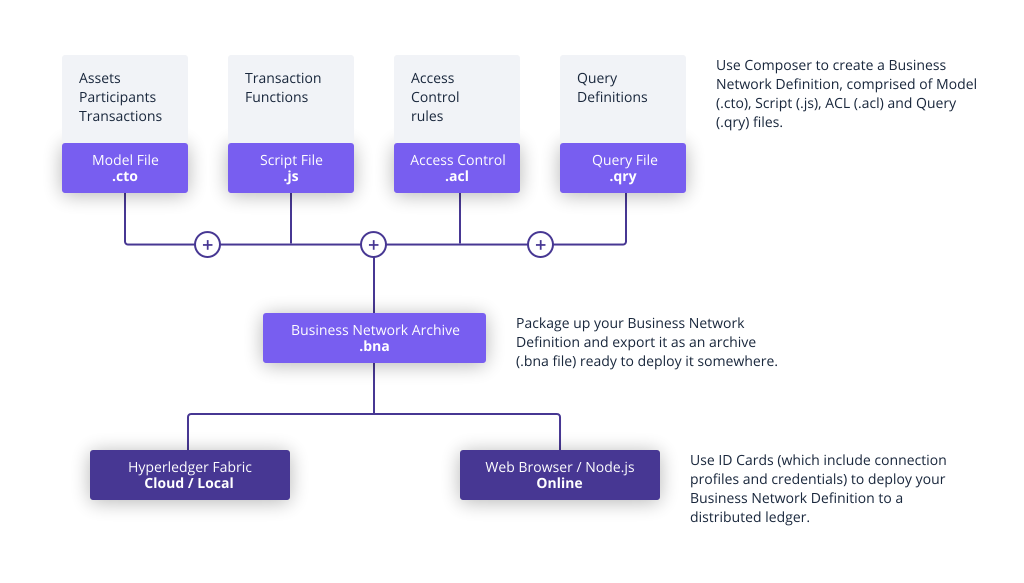
\includegraphics[width=\textwidth]{graphics/Composer-Diagram.png}
    		\caption[Zusammensetzung einer Hyperledger Composer-Applikation]{Zusammensetzung einer Hyperledger Composer-Applikation\cite{ComposerDocs}}
    		\label{fig:composer_arch}
    	\end{figure}
        
        
        
        
 %%%%%%%%%%%%%%%%%%%%%%%%%%%%%%%%%%%%%%%%%%%%%%%%%%%%%%%%%%%%%%%%%%%%%%%%%%%%%%%%%%%%       
        \begin{itemize}[noitemsep]
            \item Möglichkeit eine \gls{rest}-\gls{api} pro Business Network Card mit folgenden Features zu generieren
                \begin{itemize}[noitemsep]
                    \item Nutzung von API-Keys für die Sicherung der \gls{rest}-\gls{api}
                    \item Authentifizierung via Passport auf Linux-Maschinen
                    \item ,,Explorer Test Interface``, welches automatisch generiert wird und essentiell eine Dokumentation der \gls{api} darstellt mit der zusätzlichen Möglichkeit die \gls{api}-Calls zu testen.
                    \item Key für dynamisches Logging
                    \item Event Publication via WebSocket
                    \item \gls{tls} und HTTPS für die \gls{api}
                \end{itemize}
            \item Actors im Netzwerk (Peers, Orderers, Client Applications etc. haben eine digitale Identität, welche sich in einem X.509 digitalem Zeritifikat befindet.
                Die Zertifikate sind letztendlich ausschlaggebend für die Zugriffskontrolle und den Rechten, die eine Entität in dem Netzwerk erhält. 
                Zusätzlich können weitere Attribute, die zu einer Identät gehören genutzt werden (wie bspw. Organisiation, Rolle, etc.), welche eine Rolle bei der Bestimmung, welche Rechte diese Entität erhalten soll, spielen können.
            \item Zertifikate kommen von einer vertrausenswürdigen Autortität, dem \gls{msp}. 
                Gleicht einer PKI mit digitalen Zertifikaten, public/\-private Keys, CA und CRL
            \item öffentliche und private Kanäle: Nachrichtenwege, um Privatsphäre von Transaktionen und Vertraulichkeit zu gewährleisten.
                Private Kanäle sind nur für bestimmte Netzwerkmitglieder sichtbar, denen der Channel freigegeben wurde.
            \item Ordering Service: ein oder mehrere Knoten, die Transaktionen in einem Block ordnen
        \end{itemize}
        
        \begin{itemize}[noitemsep]
            \item Single Organization 
            \item Membership Provider Service
        \end{itemize}
        
        Konfiguration des Frameworks
        \begin{itemize}[noitemsep]
            \item How to ensure a consistent state across all entities?...
            \item Hyperledger bietet CA für Identitäten, Authentifizierung \textrightarrow\ wie ist das bei Composer?
            \item \begin{itemize}
                \item erlaubt Sicherheitseinstellungen beim Erstellen des \gls{rest}-\gls{api}-Servers
                \item API Key
                \item Authentication mit Passport
                \item explorer Test interface ?
                \item dynamic logging
                \item event publication over websockets
                \item TLS enable/\-disable
                \item Chaincode erklären
            \end{itemize}
        \end{itemize}
    

\begin{enumerate}
    \item PeerAdmin ist für Hyperledger Instanz verantwortlich, stellt ID cards für BNA aus und entzieht dieser auch wieder, deployed business networks
    \item BNA: update network, create, issue and revoke ID cards for participants
\end{enumerate}
